\documentclass{standalone}
\usepackage{tikz}
\usetikzlibrary{patterns, positioning}

\begin{document}
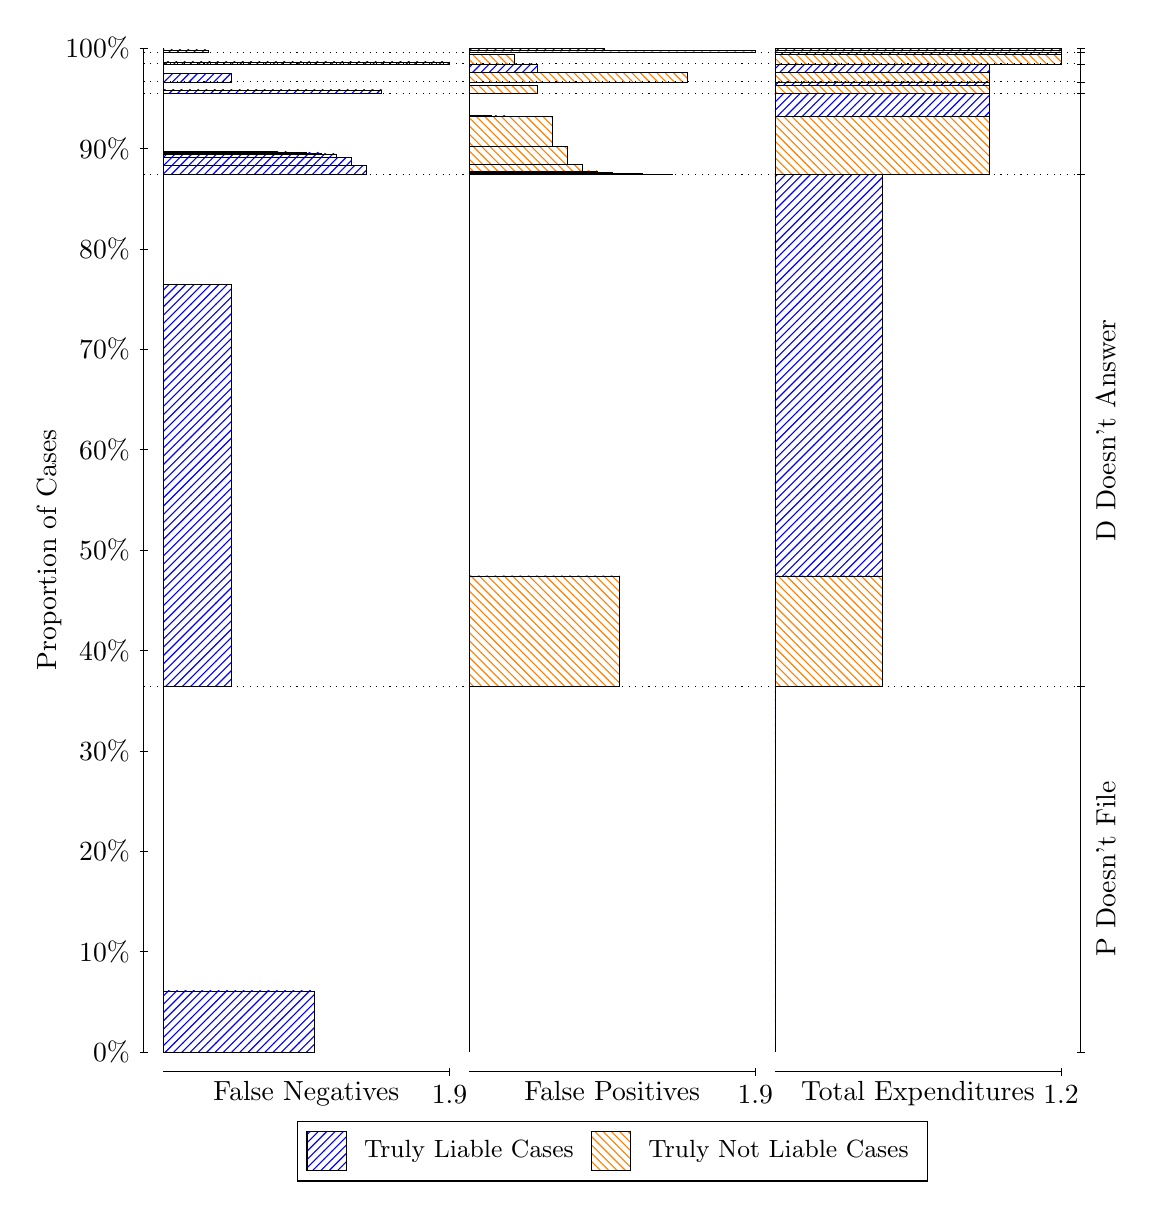
\begin{tikzpicture}
\draw[black, very thin] (1.5,1.75) -- (1.5,14.5);
\node[rotate=90, anchor=center] at (0.3, 8.125) {Proportion of Cases};
\draw[black, very thin] (1.45,1.75) -- (1.55,1.75);
\node[anchor=east] at (1.45, 1.75) {0\%};
\draw[black, very thin] (1.45,3.025) -- (1.55,3.025);
\node[anchor=east] at (1.45, 3.025) {10\%};
\draw[black, very thin] (1.45,4.3) -- (1.55,4.3);
\node[anchor=east] at (1.45, 4.3) {20\%};
\draw[black, very thin] (1.45,5.575) -- (1.55,5.575);
\node[anchor=east] at (1.45, 5.575) {30\%};
\draw[black, very thin] (1.45,6.85) -- (1.55,6.85);
\node[anchor=east] at (1.45, 6.85) {40\%};
\draw[black, very thin] (1.45,8.125) -- (1.55,8.125);
\node[anchor=east] at (1.45, 8.125) {50\%};
\draw[black, very thin] (1.45,9.4) -- (1.55,9.4);
\node[anchor=east] at (1.45, 9.4) {60\%};
\draw[black, very thin] (1.45,10.675) -- (1.55,10.675);
\node[anchor=east] at (1.45, 10.675) {70\%};
\draw[black, very thin] (1.45,11.95) -- (1.55,11.95);
\node[anchor=east] at (1.45, 11.95) {80\%};
\draw[black, very thin] (1.45,13.225) -- (1.55,13.225);
\node[anchor=east] at (1.45, 13.225) {90\%};
\draw[black, very thin] (1.45,14.5) -- (1.55,14.5);
\node[anchor=east] at (1.45, 14.5) {100\%};

\draw[black, very thin] (13.4,1.75) -- (13.4,14.5);
\draw[black, very thin] (13.35,1.75) -- (13.45,1.75);
\node[anchor=west] at (13.35, 1.75) {};
\draw[black, very thin] (13.35,6.3958) -- (13.45,6.3958);
\node[anchor=west] at (13.35, 6.3958) {};
\draw[black, very thin] (13.35,12.896) -- (13.45,12.896);
\node[anchor=west] at (13.35, 12.896) {};
\draw[black, very thin] (13.35,13.927) -- (13.45,13.927);
\node[anchor=west] at (13.35, 13.927) {};
\draw[black, very thin] (13.35,14.071) -- (13.45,14.071);
\node[anchor=west] at (13.35, 14.071) {};
\draw[black, very thin] (13.35,14.298) -- (13.45,14.298);
\node[anchor=west] at (13.35, 14.298) {};
\draw[black, very thin] (13.35,14.444) -- (13.45,14.444);
\node[anchor=west] at (13.35, 14.444) {};
\draw[black, very thin] (13.35,14.5) -- (13.45,14.5);
\node[anchor=west] at (13.35, 14.5) {};

\draw[black, very thin, pattern color=blue, pattern=north east lines] (1.75,1.75) rectangle (3.6623,2.525);
\draw[black, very thin, pattern color=orange, pattern=north west lines] (1.75,2.525) rectangle (1.75,6.3958);
\draw[black, very thin, pattern color=blue, pattern=north east lines] (1.75,6.3958) rectangle (2.6105,11.495);
\draw[black, very thin, pattern color=orange, pattern=north west lines] (1.75,11.495) rectangle (1.75,12.896);
\draw[black, very thin, pattern color=blue, pattern=north east lines] (1.75,12.896) rectangle (4.3316,13.013);
\draw[black, very thin, pattern color=blue, pattern=north east lines] (1.75,13.013) rectangle (4.1404,13.115);
\draw[black, very thin, pattern color=blue, pattern=north east lines] (1.75,13.115) rectangle (3.9491,13.155);
\draw[black, very thin, pattern color=blue, pattern=north east lines] (1.75,13.155) rectangle (3.7579,13.164);
\draw[black, very thin, pattern color=blue, pattern=north east lines] (1.75,13.164) rectangle (3.7579,13.167);
\draw[black, very thin, pattern color=blue, pattern=north east lines] (1.75,13.167) rectangle (3.5667,13.177);
\draw[black, very thin, pattern color=blue, pattern=north east lines] (1.75,13.177) rectangle (3.3754,13.18);
\draw[black, very thin, pattern color=blue, pattern=north east lines] (1.75,13.18) rectangle (3.1842,13.185);
\draw[black, very thin, pattern color=blue, pattern=north east lines] (1.75,13.185) rectangle (2.993,13.189);
\draw[black, very thin, pattern color=blue, pattern=north east lines] (1.75,13.189) rectangle (2.8018,13.191);
\draw[black, very thin, pattern color=orange, pattern=north west lines] (1.75,13.191) rectangle (1.75,13.927);
\draw[black, very thin, pattern color=blue, pattern=north east lines] (1.75,13.927) rectangle (4.5228,13.968);
\draw[black, very thin, pattern color=orange, pattern=north west lines] (1.75,13.968) rectangle (1.75,14.071);
\draw[black, very thin, pattern color=blue, pattern=north east lines] (1.75,14.071) rectangle (2.6105,14.178);
\draw[black, very thin, pattern color=orange, pattern=north west lines] (1.75,14.178) rectangle (1.75,14.298);
\draw[black, very thin, pattern color=blue, pattern=north east lines] (1.75,14.298) rectangle (5.3833,14.324);
\draw[black, very thin, pattern color=orange, pattern=north west lines] (1.75,14.324) rectangle (1.75,14.444);
\draw[black, very thin, pattern color=blue, pattern=north east lines] (1.75,14.444) rectangle (2.3237,14.475);
\draw[black, very thin, pattern color=orange, pattern=north west lines] (1.75,14.475) rectangle (1.75,14.5);
\draw[black, very thin, pattern color=orange, pattern=north west lines] (5.6333,1.75) rectangle (5.6333,5.6208);
\draw[black, very thin, pattern color=blue, pattern=north east lines] (5.6333,5.6208) rectangle (5.6333,6.3958);
\draw[black, very thin, pattern color=orange, pattern=north west lines] (5.6333,6.3958) rectangle (7.5456,7.7968);
\draw[black, very thin, pattern color=blue, pattern=north east lines] (5.6333,7.7968) rectangle (5.6333,12.896);
\draw[black, very thin, pattern color=orange, pattern=north west lines] (5.6333,12.896) rectangle (8.2149,12.898);
\draw[black, very thin, pattern color=orange, pattern=north west lines] (5.6333,12.898) rectangle (8.0237,12.9);
\draw[black, very thin, pattern color=orange, pattern=north west lines] (5.6333,12.9) rectangle (7.8325,12.904);
\draw[black, very thin, pattern color=orange, pattern=north west lines] (5.6333,12.904) rectangle (7.6412,12.909);
\draw[black, very thin, pattern color=orange, pattern=north west lines] (5.6333,12.909) rectangle (7.45,12.924);
\draw[black, very thin, pattern color=orange, pattern=north west lines] (5.6333,12.924) rectangle (7.2588,12.927);
\draw[black, very thin, pattern color=orange, pattern=north west lines] (5.6333,12.927) rectangle (7.2588,12.941);
\draw[black, very thin, pattern color=orange, pattern=north west lines] (5.6333,12.941) rectangle (7.0675,13.021);
\draw[black, very thin, pattern color=orange, pattern=north west lines] (5.6333,13.021) rectangle (6.8763,13.253);
\draw[black, very thin, pattern color=orange, pattern=north west lines] (5.6333,13.253) rectangle (6.6851,13.632);
\draw[black, very thin, pattern color=blue, pattern=north east lines] (5.6333,13.632) rectangle (6.3026,13.634);
\draw[black, very thin, pattern color=blue, pattern=north east lines] (5.6333,13.634) rectangle (6.1114,13.638);
\draw[black, very thin, pattern color=blue, pattern=north east lines] (5.6333,13.638) rectangle (5.9202,13.643);
\draw[black, very thin, pattern color=blue, pattern=north east lines] (5.6333,13.643) rectangle (5.7289,13.647);
\draw[black, very thin, pattern color=blue, pattern=north east lines] (5.6333,13.647) rectangle (5.6333,13.927);
\draw[black, very thin, pattern color=orange, pattern=north west lines] (5.6333,13.927) rectangle (6.4939,14.03);
\draw[black, very thin, pattern color=blue, pattern=north east lines] (5.6333,14.03) rectangle (5.6333,14.071);
\draw[black, very thin, pattern color=orange, pattern=north west lines] (5.6333,14.071) rectangle (8.4061,14.19);
\draw[black, very thin, pattern color=blue, pattern=north east lines] (5.6333,14.19) rectangle (6.4939,14.298);
\draw[black, very thin, pattern color=orange, pattern=north west lines] (5.6333,14.298) rectangle (6.207,14.418);
\draw[black, very thin, pattern color=blue, pattern=north east lines] (5.6333,14.418) rectangle (5.6333,14.444);
\draw[black, very thin, pattern color=orange, pattern=north west lines] (5.6333,14.444) rectangle (9.2667,14.469);
\draw[black, very thin, pattern color=blue, pattern=north east lines] (5.6333,14.469) rectangle (7.3544,14.5);
\draw[black, very thin, pattern color=orange, pattern=north west lines] (9.5167,1.75) rectangle (9.5167,5.6208);
\draw[black, very thin, pattern color=blue, pattern=north east lines] (9.5167,5.6208) rectangle (9.5167,6.3958);
\draw[black, very thin, pattern color=orange, pattern=north west lines] (9.5167,6.3958) rectangle (10.879,7.7968);
\draw[black, very thin, pattern color=blue, pattern=north east lines] (9.5167,7.7968) rectangle (10.879,12.896);
\draw[black, very thin, pattern color=orange, pattern=north west lines] (9.5167,12.896) rectangle (12.242,12.898);
\draw[black, very thin, pattern color=blue, pattern=north east lines] (9.5167,12.898) rectangle (12.242,12.9);
\draw[black, very thin, pattern color=orange, pattern=north west lines] (9.5167,12.9) rectangle (12.242,13.63);
\draw[black, very thin, pattern color=blue, pattern=north east lines] (9.5167,13.63) rectangle (12.242,13.919);
\draw[black, very thin, pattern color=orange, pattern=north west lines] (9.5167,13.919) rectangle (12.242,13.924);
\draw[black, very thin, pattern color=blue, pattern=north east lines] (9.5167,13.924) rectangle (12.242,13.927);
\draw[black, very thin, pattern color=orange, pattern=north west lines] (9.5167,13.927) rectangle (12.242,14.03);
\draw[black, very thin, pattern color=blue, pattern=north east lines] (9.5167,14.03) rectangle (12.242,14.071);
\draw[black, very thin, pattern color=orange, pattern=north west lines] (9.5167,14.071) rectangle (12.242,14.19);
\draw[black, very thin, pattern color=blue, pattern=north east lines] (9.5167,14.19) rectangle (12.242,14.298);
\draw[black, very thin, pattern color=orange, pattern=north west lines] (9.5167,14.298) rectangle (13.15,14.418);
\draw[black, very thin, pattern color=blue, pattern=north east lines] (9.5167,14.418) rectangle (13.15,14.444);
\draw[black, very thin, pattern color=orange, pattern=north west lines] (9.5167,14.444) rectangle (13.15,14.469);
\draw[black, very thin, pattern color=blue, pattern=north east lines] (9.5167,14.469) rectangle (13.15,14.5);
\draw[black, dotted] (1.5,6.3958) -- (13.4,6.3958);
\draw[black, dotted] (1.5,12.896) -- (13.4,12.896);
\draw[black, dotted] (1.5,13.927) -- (13.4,13.927);
\draw[black, dotted] (1.5,14.071) -- (13.4,14.071);
\draw[black, dotted] (1.5,14.298) -- (13.4,14.298);
\draw[black, dotted] (1.5,14.444) -- (13.4,14.444);
\draw[black, very thin] (1.75,1.5) -- (5.3833,1.5);
\node[anchor=north] at (3.5667, 1.5) {False Negatives};
\draw[black, very thin] (5.3833,1.45) -- (5.3833,1.55);
\node[anchor=north] at (5.3833, 1.45) {1.9};

\draw[black, very thin] (5.6333,1.5) -- (9.2667,1.5);
\node[anchor=north] at (7.45, 1.5) {False Positives};
\draw[black, very thin] (9.2667,1.45) -- (9.2667,1.55);
\node[anchor=north] at (9.2667, 1.45) {1.9};

\draw[black, very thin] (9.5167,1.5) -- (13.15,1.5);
\node[anchor=north] at (11.333, 1.5) {Total Expenditures};
\draw[black, very thin] (13.15,1.45) -- (13.15,1.55);
\node[anchor=north] at (13.15, 1.45) {1.2};

\node[black, centered, rotate=90] at (13.72, 4.0729) {P Doesn't File};
\node[black, centered, rotate=90] at (13.72, 9.6461) {D Doesn't Answer};






\draw (7.449999999999999,1.5) node[draw=none] (baseCoordinate) {};
\begin{scope}[align=center]
        \matrix[scale=0.5, draw=black, below=0.5cm of baseCoordinate, nodes={draw}, column sep=0.1cm]{
            \node[rectangle, draw, minimum width=0.5cm, minimum height=0.5cm, pattern=north east lines, pattern color=blue] {}; &
            \node[draw=none, font=\small] (B) {Truly Liable Cases}; &
            \node[rectangle, draw, minimum width=0.5cm, minimum height=0.5cm, pattern=north west lines, pattern color=orange] {}; &
            \node[draw=none, font=\small] (B) {Truly Not Liable Cases}; \\
            };
\end{scope}

\end{tikzpicture}
\end{document}